%===================================== CHAP 5 =================================

\chapter{Implementation}

\figurename~\ref{fig:architecture-overview} shows a high level overview of the
CARP hardware platform extended with a readout module. While the system has been
extended with new functionality and partially ported to Chisel, the overall
architecture of the system has been largely preserved. In
\figurename~\ref{fig:architecture-detail}, a more detailed view of the system is
shown. Modules are annotated with either a C(hisel) or a V(HDL) in the upper
right corner to indicate their porting status. The top level logic and wiring
gluing all the modules together is all done in Chisel.

\begin{figure}[ht]
  \centering
  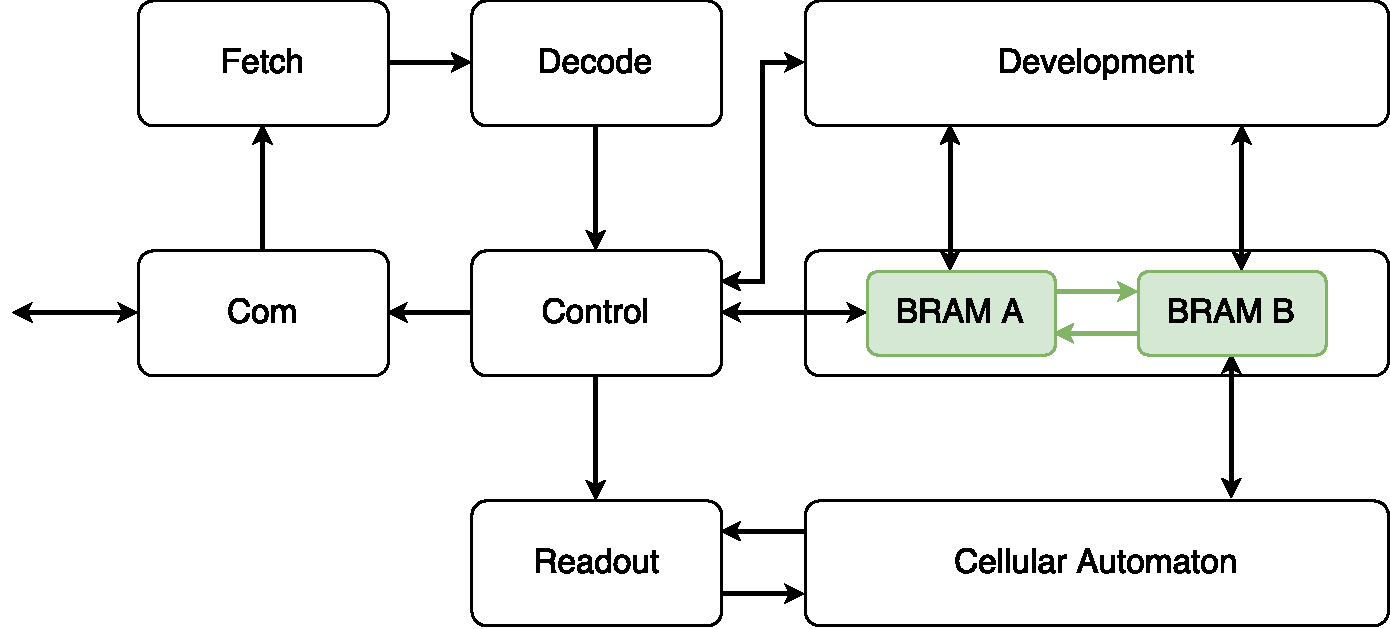
\includegraphics[width=0.8\linewidth]{fig/architecture-overview}
  \caption{
    Block diagram of the CARP hardware architecture extended with a readout layer.
  }
  \label{fig:architecture-overview}
\end{figure}

\begin{sidewaysfigure}[ht]
    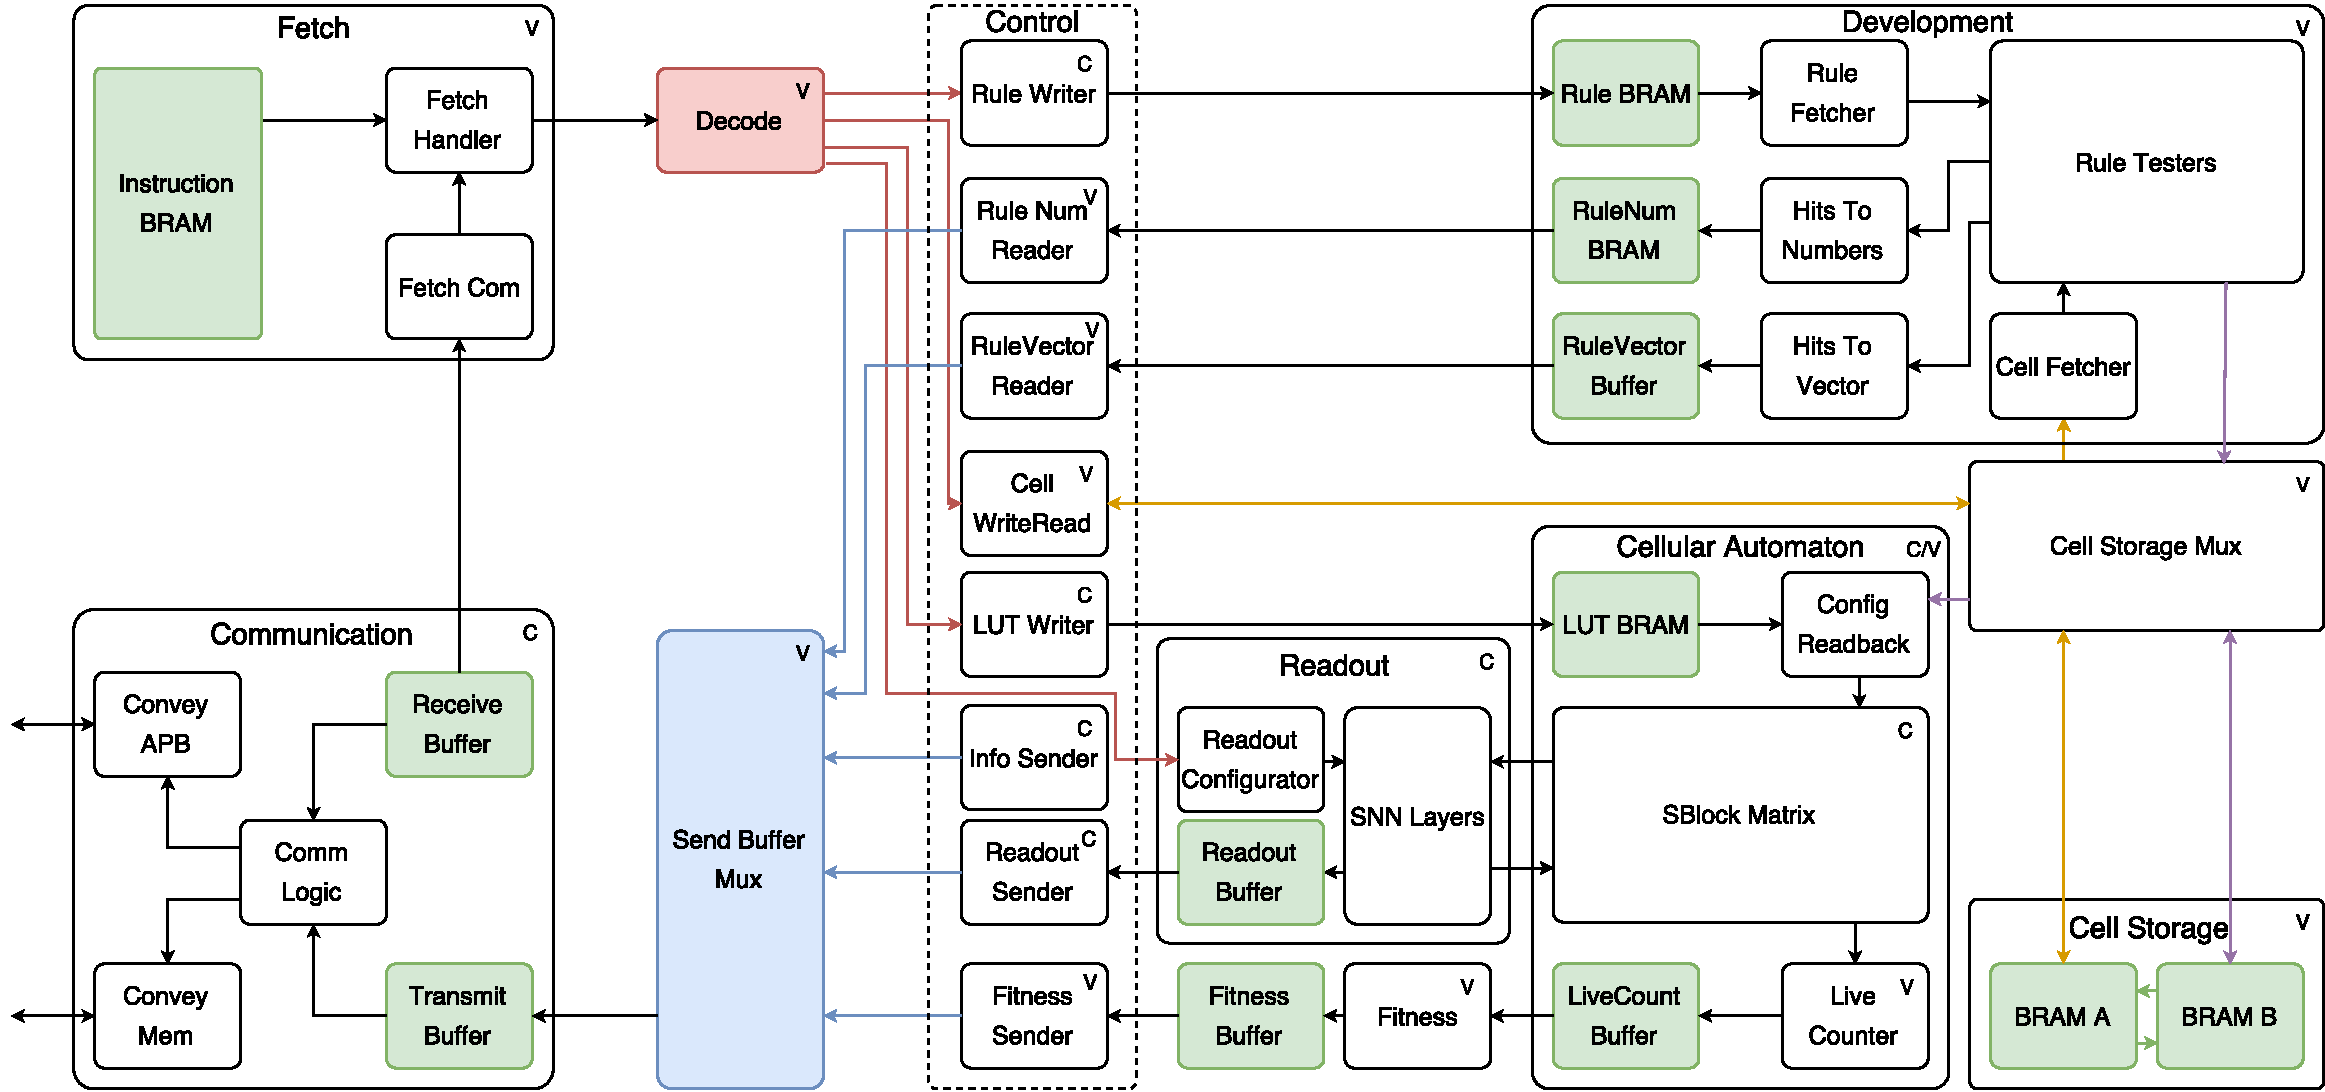
\includegraphics[width=\textwidth]{fig/architecture-detail}
    \caption{
      Modified reprint from~\cite{Lundal2015a} showing a detailed overview of
      the CARP architecture and its constituent modules. Modules annotated with a C in
      the upper right corner are implemented in / have been ported to Chisel, while
      those annotated with a V are implemented in VHDL. Child modules not annotated
      are implemented in the same language as their parent modules. Signals indicate
      flow of data or direction of communication, control signals and detailed
      interfaces are ommited for clarity.
    }
    \label{fig:architecture-detail}
\end{sidewaysfigure}

\section{General overview}

This section gives an overview of the platform as a whole, as well as insight
into the functionality of t

The CARP hardware platform operates in a three-stage, interlocked pipeline. The
stages are Fetch, Decode and Execute. In the execute stage, an instruction can
utilize the CA module, Development module or any of the Control modules. The
readout module

\section{Communication}

The Convey coprocessor connects to the host computer via PCIe. 

\section{Readout}

\section{Cellular Automata}

\section{Parameterization}

\section{Software API}

\cleardoublepage
%%% Local Variables:
%%% mode: latex
%%% TeX-master: "../thesis"
%%% End:
